\chapter{Frontend web desplegado}\label{chap:frontend}
\section{Aplicación en AWS Amplify}
Para ASTRA CLOUD se implementó una aplicación web desplegada en AWS Amplify. La interfaz se entrega por HTTPS y tiene las secciones Inicio, Explorar, Clubes, Mis películas, Analítica y órbitas de reproducción. La Figura~\ref{fig:frontend-inicio} muestra la portada pública, con contenido destacado, tendencias y accesos a una película o a una experiencia compartida.

La consola de AWS Amplify identifica la aplicación \texttt{astra-frontend}, muestra su rama de producción conectada y ofrece el acceso a la URL desplegada. Esta captura demuestra la configuración visible del despliegue de Amplify; no representa una consulta de Athena ni constituye evidencia del Glue Data Catalog.
\begin{figure}[H]\centering
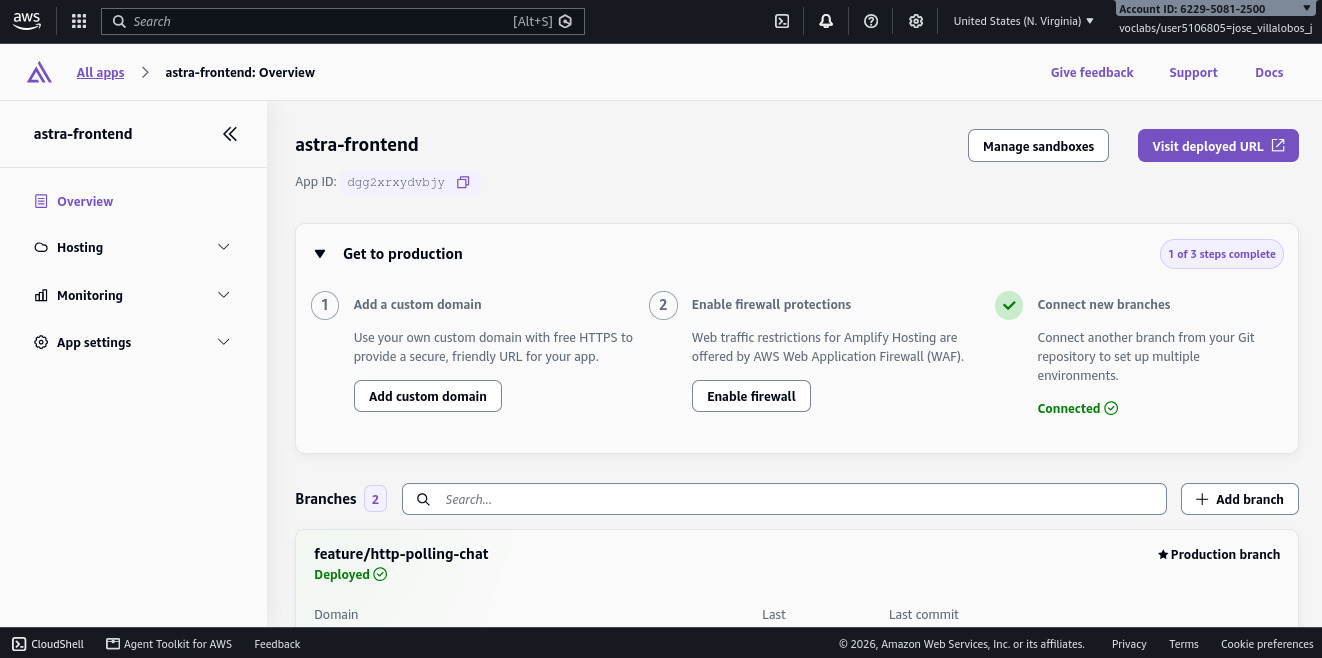
\includegraphics[width=.96\textwidth]{../evidencia_athena.jpeg}
\caption{Aplicación \texttt{astra-frontend} y rama de producción visibles en AWS Amplify.}
\label{fig:amplify-frontend-evidencia}
\end{figure}

\begin{figure}[H]\centering
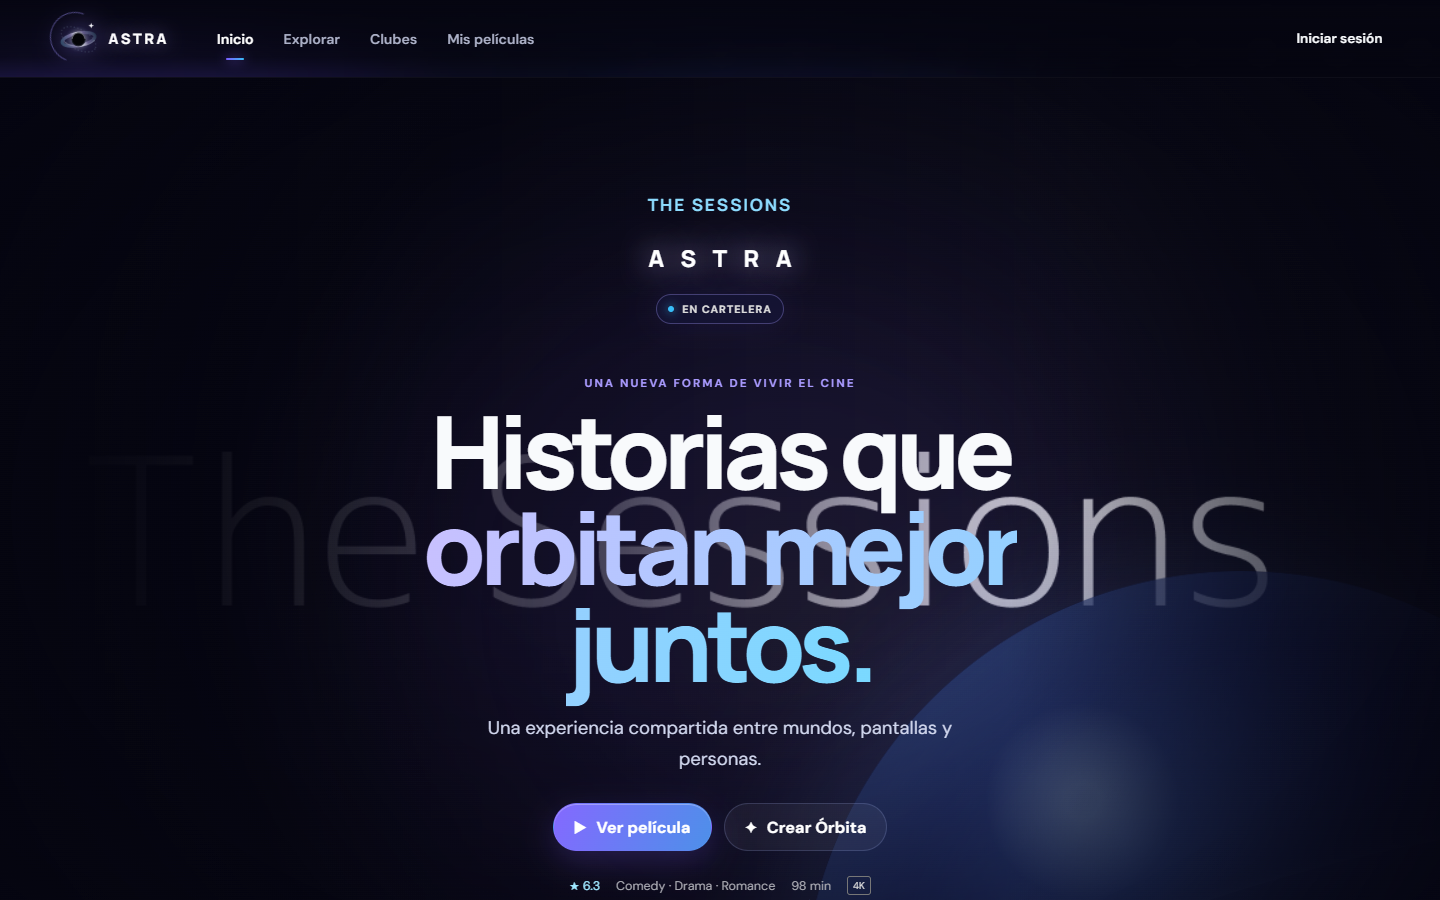
\includegraphics[width=.94\textwidth]{evidence/frontend/01-inicio-publico.png}
\caption{Inicio público de ASTRA CLOUD desplegado en AWS Amplify.}
\label{fig:frontend-inicio}
\end{figure}

El catálogo permite buscar películas y abrir su detalle. En las Figuras~\ref{fig:frontend-explorar} y~\ref{fig:frontend-detalle} se muestran la exploración, los metadatos y acciones como crear una órbita, dar like o agregar una película a la watchlist. Estas acciones requieren iniciar sesión. Durante las pruebas no se realizaron cambios en la cuenta utilizada.

\begin{figure}[H]\centering
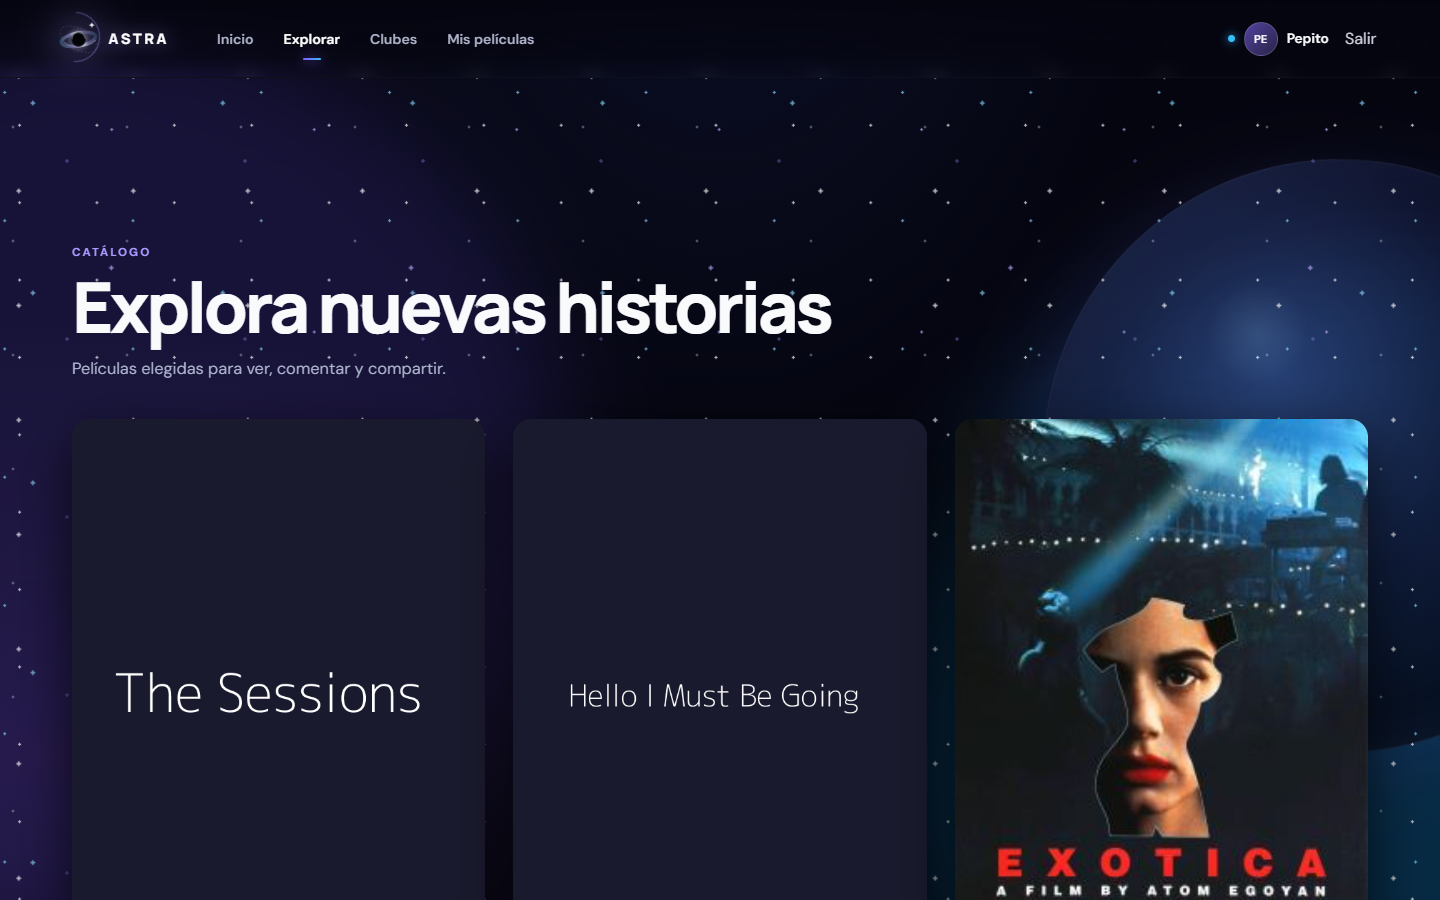
\includegraphics[width=.94\textwidth]{evidence/frontend/03-explorar.png}
\caption{Exploración del catálogo cinematográfico desde la aplicación web.}
\label{fig:frontend-explorar}
\end{figure}

\begin{figure}[H]\centering
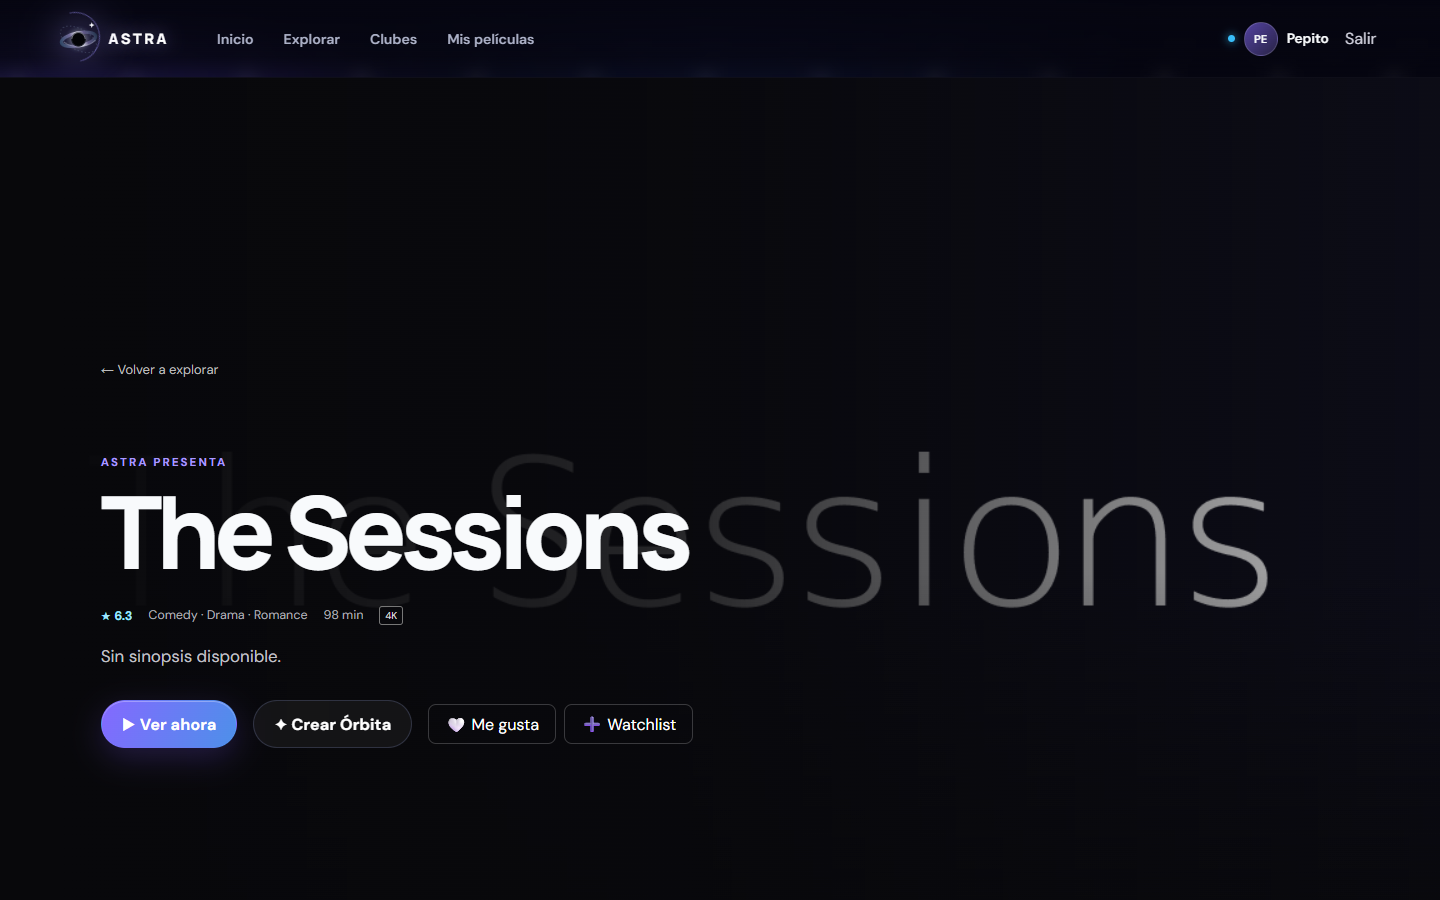
\includegraphics[width=.94\textwidth]{evidence/frontend/04-detalle-pelicula.png}
\caption{Detalle de película con acciones de reproducción, órbita, like y watchlist.}
\label{fig:frontend-detalle}
\end{figure}

\section{Comunidad y sesión compartida}
Desde la interfaz se pueden consultar clubes y unirse a una comunidad, como se muestra en la Figura~\ref{fig:frontend-clubes}. Para ver una película en grupo, la pantalla de la Figura~\ref{fig:frontend-sesion} reúne el reproductor, los participantes, el chat en vivo y los controles de reacción. Esta parte usa Cinema Session junto con los datos de Community.

\begin{figure}[H]\centering
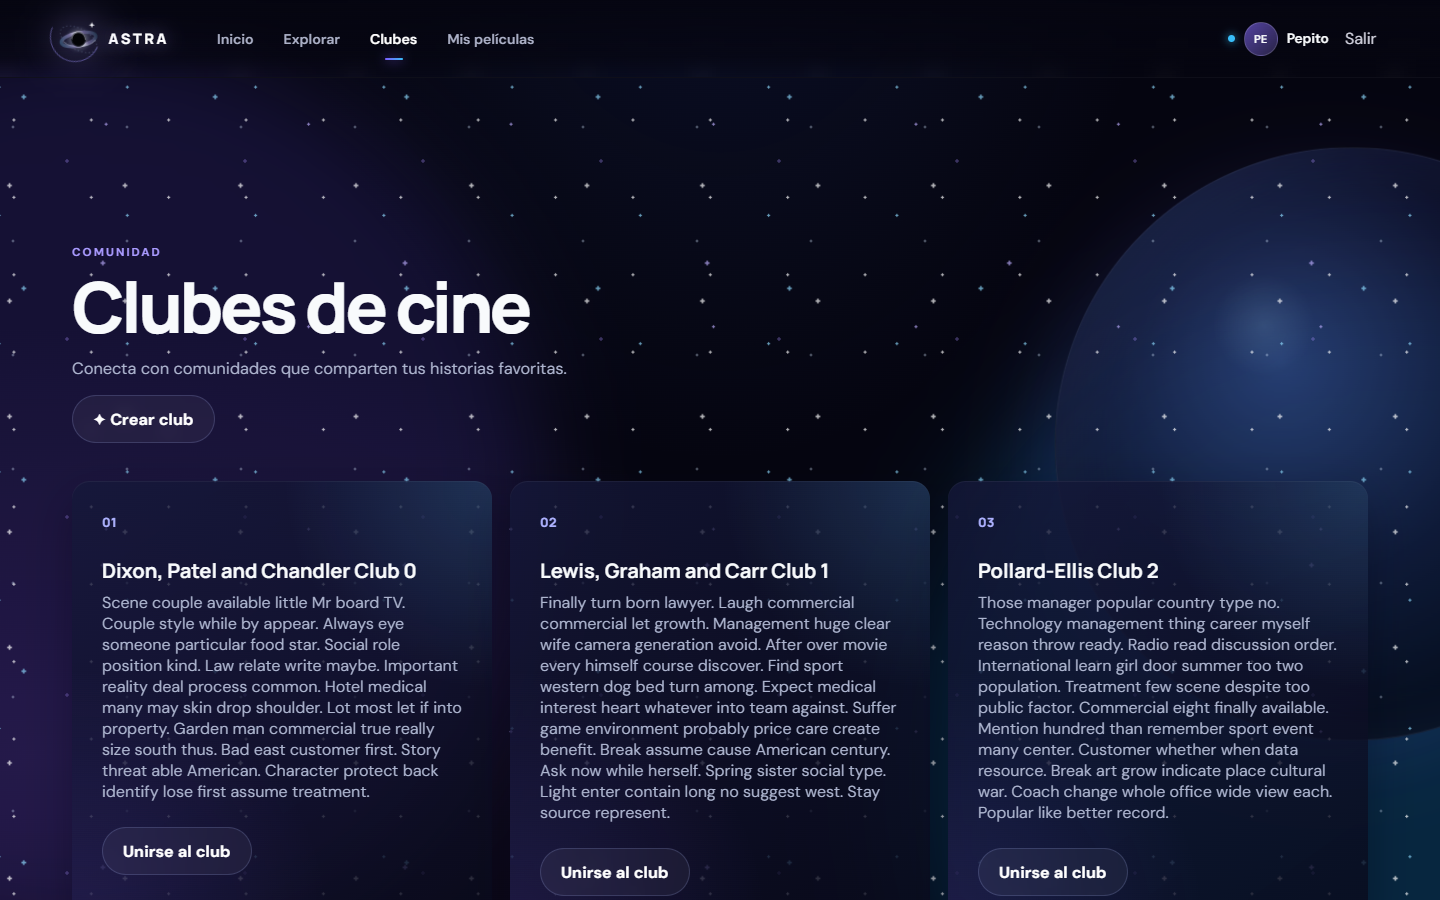
\includegraphics[width=.94\textwidth]{evidence/frontend/05-clubes.png}
\caption{Listado de clubes y acceso a las acciones comunitarias.}
\label{fig:frontend-clubes}
\end{figure}

\begin{figure}[H]\centering
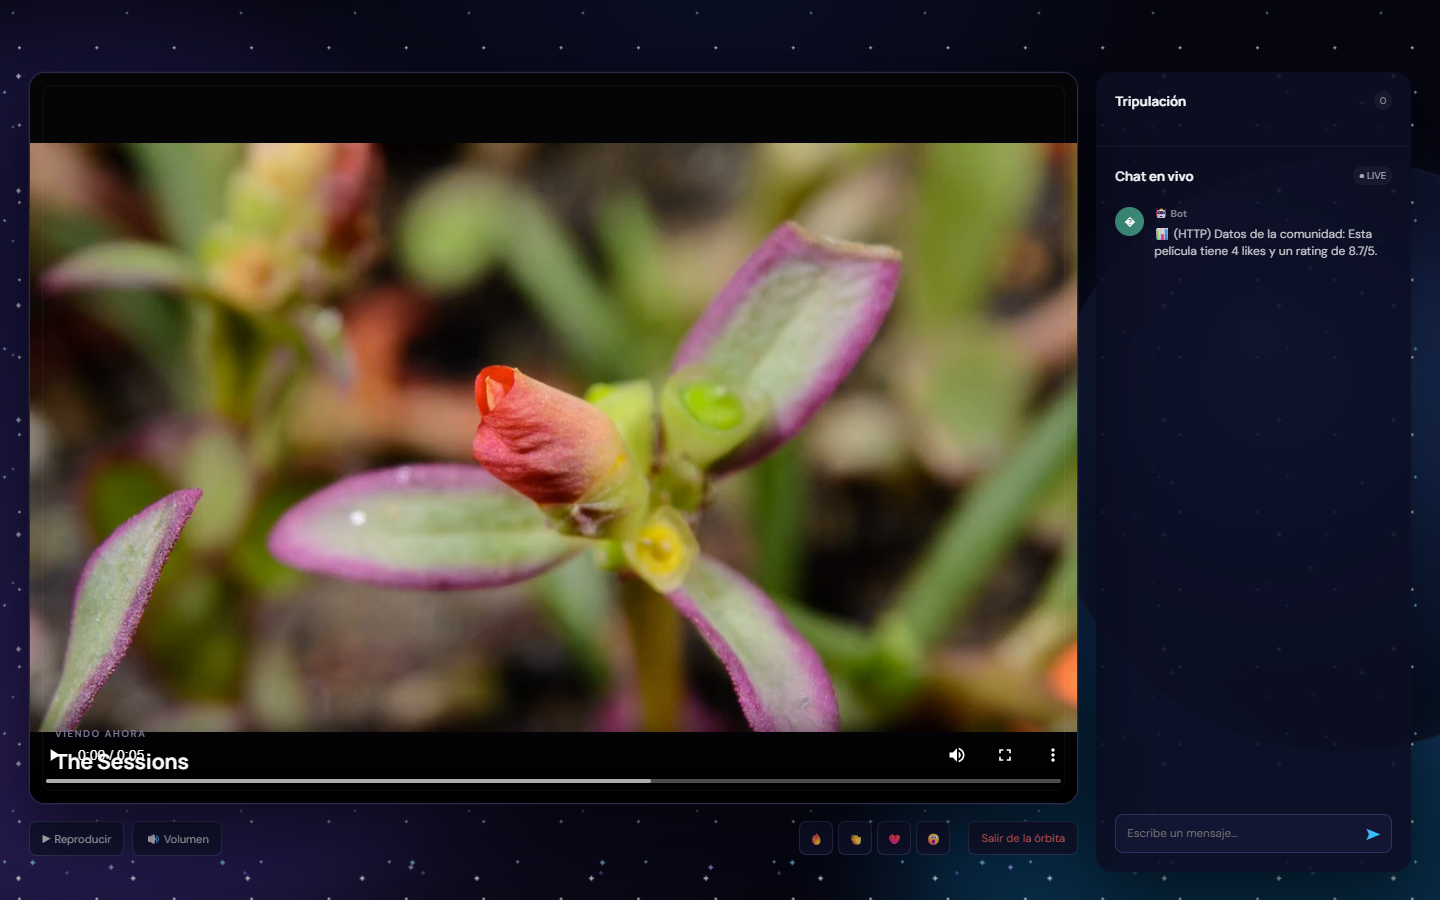
\includegraphics[width=.94\textwidth]{evidence/frontend/07-sesion-cine.png}
\caption{Órbita de cine con reproductor, chat en vivo y controles de la sesión.}
\label{fig:frontend-sesion}
\end{figure}

\section{Consumo de servicios}
La configuración y el paquete JavaScript publicados por Amplify contienen las seis URL de API Gateway. La trazabilidad se verificó además contra la rama \texttt{origin/feature/http-polling-chat} del frontend, compatible con los controladores de los repositorios locales. La Tabla~\ref{tab:frontend-servicios} registra dos operaciones REST implementadas para cada servicio; ``código/bundle'' indica que la operación está presente tanto en el código de esa rama como en el paquete desplegado, y no que se ejecutó una operación que modifica datos durante la revisión.
El bundle define \texttt{POST /api/auth/login} y \texttt{GET /api/v1/users/me}; la navegación pública observó la carga de \texttt{GET /api/catalog/movies} en Explorar. Las pantallas de detalle, clubes y sesión están disponibles en la interfaz, pero las operaciones protegidas no se marcan como ejecutadas cuando dependen de autenticación no completada. La Tabla~\ref{tab:frontend-servicios} distingue este alcance de verificación.

\begin{table}[H]\centering\small\renewcommand{\arraystretch}{1.22}
\caption{Trazabilidad frontend -- REST -- microservicio.}\label{tab:frontend-servicios}
\begin{tabularx}{\textwidth}{p{.15\textwidth}p{.32\textwidth}Y}
\toprule Servicio & Acción, archivo frontend y operaciones REST & Verificación realizada \\\midrule
Identity & \texttt{authApi.ts}: iniciar sesión/registro; \texttt{POST /api/auth/login}, \texttt{POST /api/auth/register}. & Implementadas en el código y en el paquete desplegado; durante esta revisión no se confirmó el inicio de sesión desde la interfaz. \\
Catalog & \texttt{catalogApi.ts}: inicio, explorar y órbita; \texttt{GET /api/catalog/movies}, \path{GET /api/catalog/movies/\{id\}/session-info}. & Implementadas en el código y en el paquete desplegado; la consulta del catálogo se observó desde la interfaz. \\
Community & \texttt{communityApi.ts}: clubes/unirse; \texttt{GET /api/v1/clubs}, \texttt{POST /api/v1/clubs/\{id\}/members}. & Implementadas en el código y en el paquete desplegado; durante la revisión no se ejecutaron operaciones que modificaran datos. \\
Interaction & \texttt{MovieDetail}: likes y watchlist; \texttt{GET /users/\{id\}/likes}, \texttt{GET /users/\{id\}/watchlist}. & Implementadas en el código y en el paquete desplegado; durante la revisión no se ejecutaron acciones que modificaran datos. \\
Cinema Session & \texttt{useCinemaRoom.ts}: sincronización/chat; \texttt{GET /api/v1/sessions/\{id\}/state}, \texttt{POST /api/v1/sessions/\{id\}/chat}. & Implementadas en el código y en el paquete desplegado. El servicio también utiliza \texttt{PATCH /playback} para actualizar la reproducción; no se creó una sesión de prueba durante esta revisión. \\
Analytics & \texttt{analyticsService.ts}: tablero; \texttt{GET /api/v1/dashboard/kpis}, \texttt{GET /api/v1/genres/most-watched}. & Implementadas en el código y en el paquete desplegado; su ejecución desde la interfaz requiere una sesión autenticada. \\
\bottomrule
\end{tabularx}
\end{table}

La navegación pública confirmó la pantalla Explorar. El intento autorizado de iniciar sesión no completó una sesión visible y, por ello, las rutas protegidas, incluida Analytics, no se clasifican como ejecutadas en la UI. La evidencia de dos operaciones por servicio corresponde a implementación y paquete desplegado; una prueba manual autenticada que complete el login sigue siendo necesaria para demostrar su ejecución extremo a extremo.
